\chapter{Bayessche Netze - Reasoning under Uncertainty}
\section{Einführung}
Viele Probleme sind oft zu komplex, um mit ihnen intuitiv umzugehen. Deswegen muss man diese aufspalten. Bayessche Netze sind ein guter Weg, um Abhängigkeiten zwischen Wahrscheinlichkeiten zu vereinfachen.

\section{Begriffe}
\begin{itemize}
\item Sensitivität: Wieviel Prozent des Resultats sind true-positive?
\item Spezifizität: Wieviel Prozent des Resultats sind true-negative?
\item true-positive: Richtig erkannte positive Ausgänge eines Tests (Beispiel: $p(positive | HIV)$.
\item true-negative: Richtig erkannte negative Ausgänge eines Tests (Beispiel: $p(negative | \neg HIV)$.
\item false-positive: Falsch erkannte positive Ausgänge eines Tests (Beispiel: $p(positive | \neg HIV)$.
\item false-negative: Falsch erkannte negative Ausgänge eines Tests (Beispiel: $p(negative | HIV)$.
\end{itemize}

\section{From Real World to Random Variables}
Folgende Geschichte:\\
\textit{In Los Angeles sind Einbrüche und Erdbeben häufig. Beide können einen Alarm auslösen. Wenn der Alarm losgeht, kann es sein, dass mich meine Nachbarn, John oder Mary, anrufen.}

\begin{enumerate}
\item Wo sind Unsicherheiten in der Geschichte?
\item Wenn diese gefunden sind, muss man diesen sogannte Zufallsvariablen ("Random variables") zuweisen:
\begin{itemize}
\item B $\Rightarrow$ Einbruch
\item E $\Rightarrow$ Erdbeben
\item A $\Rightarrow$ Alarm
\item J $\Rightarrow$ John ruft an
\item M $\Rightarrow$ Mary ruft an
\end{itemize}
\item Danach muss man das Set der möglichen Werte jeder Variablen herausfinden (Hier nur true oder false, die Zufallsvariablen sind also binär).
\end{enumerate}

\section{Global- und Marginalverteilung}
Die multivariate Verteilung (Joint-Distribution) $P(A,B,E,J,M)$ über alle Variablen ist die \textbf{Globale Wahrscheinlichkeitsverteilung}.
Wenn diese bekannt ist, kann man daraus - durch den Vorgang der \textbf{Marginalisation} - die anderen multivariaten Verteilungen ableiten. Diese werden Marginalverteilungen genannt.

\section{Bayes Theorem}
\[
P(B_j | A) = \frac{P(B_j) P(A | B_j)}{P(A)}
\]
Sprich: Die Wahrscheinlichkeit, dass $B_j$ gegeben $A$ eintritt, ist die Wahrscheinlichkeit, dass $B_j$ eintritt mal die Wahrscheinlichkeit, dass $A$ gegeben $B_j$ eintritt, durch die Wahrscheinlichkeit, dass $A$ eintritt (Denke an das AIDS-Beispiel, die Wahrscheinlichkeit, dass jemand tatsächlich AIDS, gegeben Test ist positiv, hat, ist gleich der Wahrscheinlichkeit, überhaupt AIDS zu haben (ist ja länderspezifisch) mal der Wahrscheinlichkeit, bei AIDS überhaupt positiv getestet zu werden, durch die Wahrscheinlichkeit, positiv zu sein).

\section{Causal Relations and Causal Networks}

Hier fragt man sich eigentlich, welche Variablen von welchen abhängen. Zum obigen Beispiel lässt sich sagen, dass:

\begin{minipage}{0.49\textwidth}
\begin{itemize}
\item Über die Abhängigkeit von Einbruch oder Erdbeben nichts genaueres bekannt ist.
\item Der Alarm von Einbruch oder Erdbeben abhängt.
\item Der Anruf von Mary oder John vom Alarm abhängt.
\end{itemize}
\end{minipage}
\begin{minipage}{0.49\textwidth}
\begin{center}
\begin{tikzpicture}[->, >=stealth', auto, semithick, node distance=2cm]
\tikzstyle{every state}=[fill=white,draw=black,thick,text=black,scale=1]
\node[state]    (A)                     {A};
\node[state]    (B)[above left of=A]                     {B};
\node[state]    (E)[above right of=A]   {E};
\node[state]    (J)[below left of=A]                     {J};
\node[state]    (M)[below right of=A]   {M};
\path
(B) edge[left,right]                           (A)
(E) edge[left,right] (A)
(A) edge[left,right] (J)
(A) edge[left,right] (M);
\end{tikzpicture}
\captionof{figure}{Causal relations}
\label{fig:causalrelations}
\end{center}
\end{minipage}


\subsection{Conditional Dependency Relations}

Bedingte Abhängigkeitbeziehungen entstehen durch die in Abbildung \ref{fig:causalrelations} dargestellten Pfeile. Somit lässt sich sagen, dass die Wahrscheinlichkeit, dass A eintrifft direkt von der Wahrscheinlichkeit abhängt, ob E und B eingetroffen sind. Aus der Wahrscheinlichkeit von A lässt sich wiederum \textbf{direkt} die Wahrscheinlichkeit für J oder M berechnen. Dies wird so geschrieben:
\begin{align}
\begin{split}
P(A | E,B) &\Rightarrow \textnormal{Wahrscheinlichkeit des Alarms, gegeben Einbruch und Erdbeben}\\
P(J | A) &\Rightarrow \textnormal{Wahrscheinlichkeit, dass Mary anruft, gegeben Alarm}\\
\textnormal{usw...}
\end{split}
\end{align}

J ist also \textbf{BEDINGT UNABHÄNGIG (conditional independent)} von B, wenn der Wert von A bekannt ist.

\subsection{Factorization}
\label{sec:factorization}

Für die Faktorisierung ist es wichtig, dass die Knoten aufgezeichnet werden. Nur direkt eintreffende Pfeile haben einen Einfluss auf den Knoten (E hat zum Beispiel keinen Einfluss auf B und umgekehrt).

Dann lässt sich die folgende Faktorisierung rein optisch herleiten:
\[
P(A,B,E,J,M) = P(J | A) * P(M | A) * P(A | B, E) * P(B) * P(E)
\]
Für die Werte würde man jetzt gegebene Wahrscheinlichkeiten einsetzen.

\section{Fusion algorithm}
Der Fusion Algorithmus ist ein Algorithmus, um bedingte Wahrscheinlichkeiten ressourceneffizienter berechnen zu können. Als Input wird benötigt: 
\begin{itemize}
\item eine sogenannte Wissensbasis (knowledgebase), die am Anfang aus den faktorisierten \ref{sec:factorization} Marginalverteilungen besteht.
\item eine Eliminationssequenz (hier empfiehlt es sich meiner Meinung nach, eine Sequenz zu wählen, die am Anfang eine Variable hat, die wenig und nicht in allzu grossen Faktoren vorkommt)
\end{itemize}

Für dieses Beispiel verwenden wir das Beispiel aus den Übungen:
\begin{figure}[h!]
\center
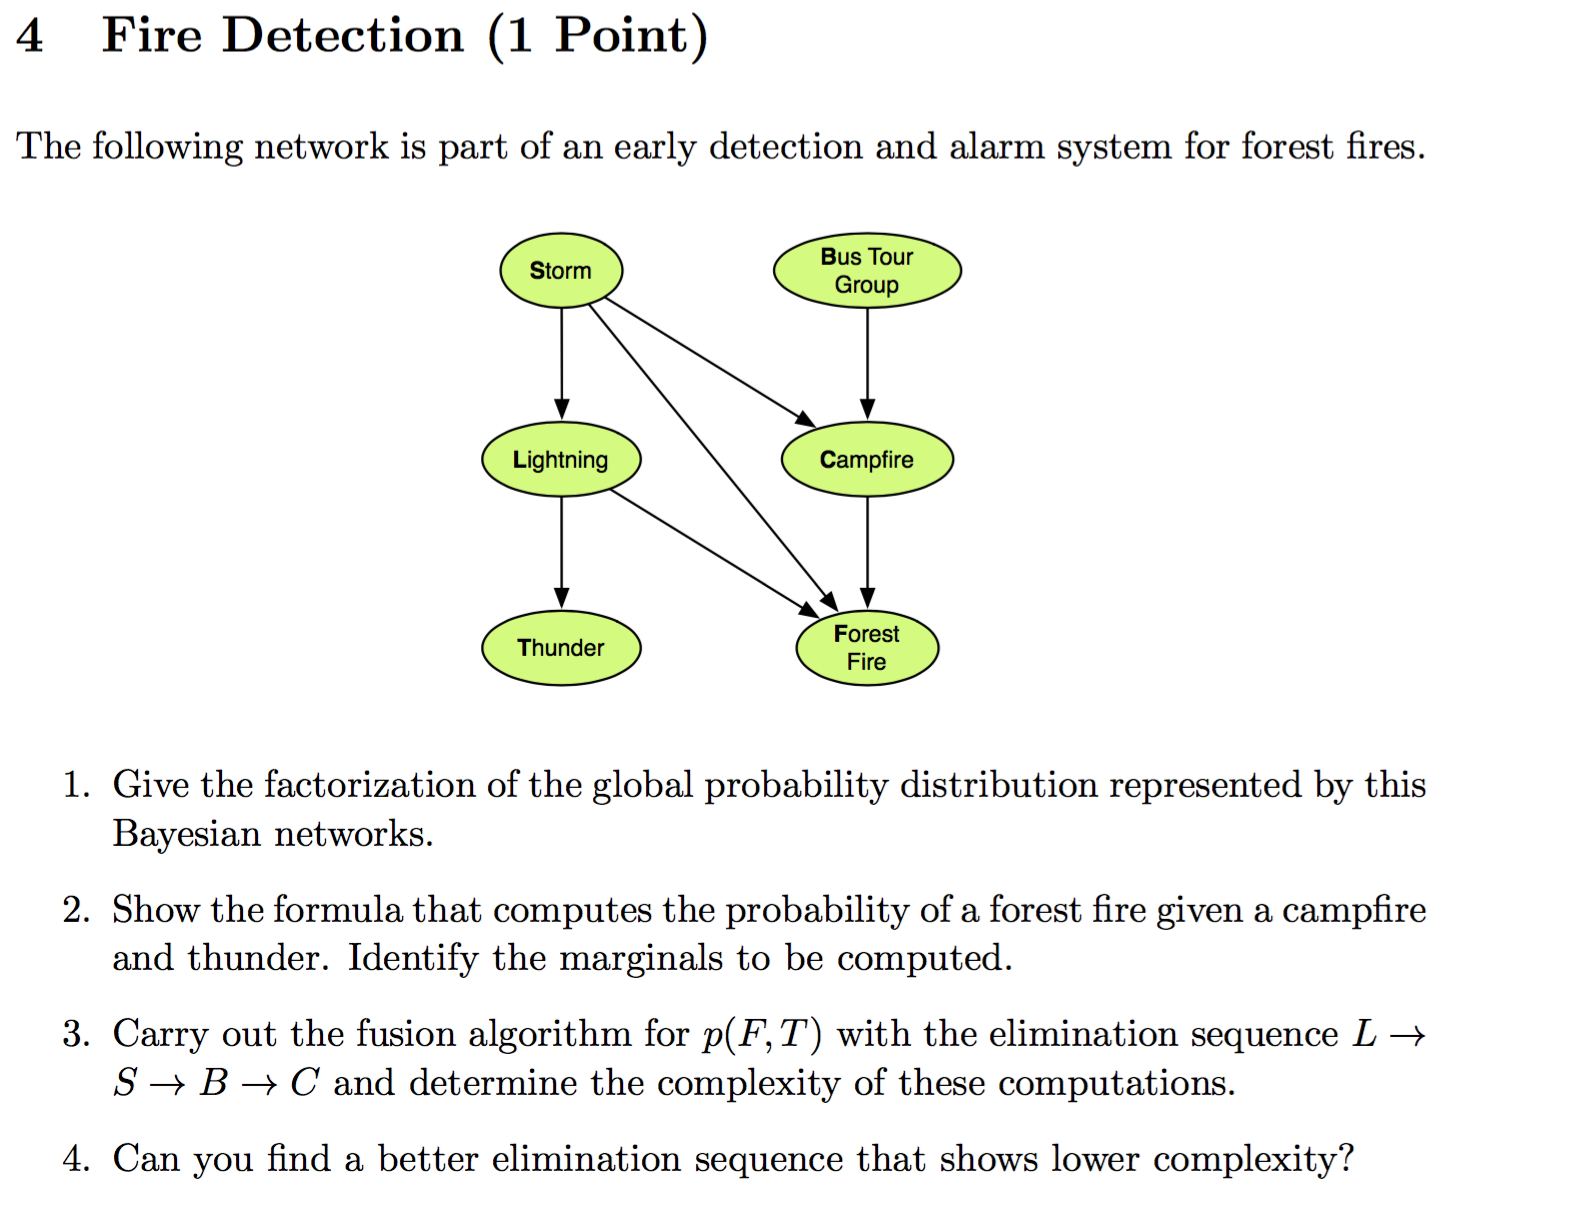
\includegraphics[width=0.9\textwidth]{fig/exercise4bayes.png}
\end{figure}

\subsection{Marginalization}
Für Aufgabe 3 mit der Eliminationssequenz $L \rightarrow S \rightarrow B \rightarrow C$ machen wir Folgendes:

\begin{enumerate}
\item Die Wissensbasis ist: $P(S, L, T, F, C, B) = P(F | C, S, L) * P(L | S) * P(T | L) * P(C | B, S) * P(S) * P(B)$

Alle Faktoren, die L enthalten summieren: $\psi_L = \sum_{\substack{L}}P(F|C,S,L) * P(L|S)*P(T|L)$

\item Die Wissenbasis hat sich verändert, die Faktoren, die L enthalten verschwinden, stattdessen wird $\psi_L$ in die Wissensbasis aufgenommen. $\psi_L$ enthält die Variablen $\{F, C, S, T\}$. Das ist wichtig, da man ja wissen muss, wann man $\psi_L$ wieder verwenden muss zur Elimination. Die Wissensbasis ist nun: $P(C | B, S) * P(S) * P(B) * \psi_L$

Nun summiert man alle Faktoren, die S enthalten: $\psi_S = \sum_{S} P(C | B, S) * P(S) * \psi_L$

\item Neue Wissensbasis: $P(B)*\psi_S$ ($\psi_S$ enthält die Variablen: $\{F,C,T,B\}$)

B entfernen: $\sum_B P(B) * \psi_S$

\item Neue Wissensbasis: $\psi_B$ ($\psi_B$ enthält die Variablen: $\{F,C,T\}$)

C entfernen: $\psi_C = \sum_C \psi_B$

$P(F,T) = \sum_{\substack{F, T}} \psi_C$
\end{enumerate}
\subsection{Back substitution}
Für die Rücksubstitution (also um die richtige Berechnungssequenz für diese Eliminationssequenz zu erhalten) geht man obige Schritte eigentlich rückwärts und setzt ein:

\begin{enumerate}
\item Ausgangslage: \\
$P(F,T) = \sum_{\substack{F, T}} \psi_C$
\item $\psi_C$ rücksubstituieren:\\
$P(F,T) = \sum_{\substack{F, T}} (\sum_C \psi_B)$
\item $\psi_B$ rücksubstituieren:\\
$P(F,T) = \sum_{\substack{F, T}} (\sum_C (\sum_B P(B) * \psi_S))$
\item $\psi_S$ rücksubstituieren:\\
$P(F,T) = \sum_{\substack{F, T}} (\sum_C (\sum_B P(B) * (\sum_{S} P(C | B, S) * P(S) * \psi_L)))$
\item $\psi_L$ rücksubstituieren:\\
$P(F,T) = \sum_{\substack{F, T}} (\sum_C (\sum_B P(B) * (\sum_{S} P(C | B, S) * P(S) * (\sum_{\substack{L}}(P(F|C,S,L) * P(L|S)*P(T|L)))))$
\end{enumerate}